\whiteBGstarBegin
\setcounter{section}{0}
\section{Trắc nghiệm}
\begin{enumerate}[label=\bfseries Câu \arabic*:]
	
	\item \mkstar{1}
	
	\cauhoi
	{Đâu không phải là một dạng cân bằng của một vật rắn?
		\begin{mcq}(2)
			\item Cân bằng bền.
			\item Cân bằng không bền.
			\item Cân bằng phiếm định.
			\item Cân bằng thẳng.
		\end{mcq}
	}
	
	\loigiai
	{	\textbf{Đáp án: D.}
		
 Các dạng cân bằng của một vật rắn: cân bằng bền, cân bằng không bền, cân bằng phiếm định.
	}
	\item \mkstar{1}
	
	\cauhoi
	{Dạng cân bằng nào dưới đây mà trọng tâm ở vị trí thấp nhất so với các vị trí lân cận?
		\begin{mcq}(2)
	\item Cân bằng bền.
	\item Cân bằng không bền.
	\item Cân bằng phiếm định.
	\item Cân bằng thẳng.
\end{mcq}
	}
	
	\loigiai
	{	\textbf{Đáp án: A.}
		
	Cân bằng bền có trọng tâm ở vị trí thấp nhất so với các vị trí lân cận.
	}
	
	\item \mkstar{1}

\cauhoi
{Dạng cân bằng nào dưới đây mà trọng tâm ở vị trí cao nhất so với các vị trí lân cận?
	\begin{mcq}(2)
		\item Cân bằng bền.
		\item Cân bằng không bền.
		\item Cân bằng phiếm định.
		\item Cân bằng thẳng.
	\end{mcq}
}

\loigiai
{	\textbf{Đáp án: B.}
	
	Cân bằng không bền có trọng tâm ở vị trí cao nhất so với các vị trí lân cận.
}
	\item \mkstar{3}
	
	\cauhoi
	{Một xe tải chở lần lượt các vật liệu sau với khối lượng bằng nhau: thép lá, gỗ và vải. Trong trường hợp nào thì xe khó bị đổ nhất?
		\begin{mcq}(2)
			\item Thép lá
			\item Gỗ.
			\item Vải.
			\item Cả 3 trường hợp như nhau.
		\end{mcq}
	}
	
	\loigiai
	{	\textbf{Đáp án: A.}
		
		Khi chở thép, trọng tâm của cả xe và hàng là thấp nhất trong các trường hợp đã cho, nên mức vững vàng của xe lớn nhất, xe khó bị đổ nhất. 
	}
	\item \mkstar{3}

\cauhoi
{Một xe tải chở lần lượt các vật liệu sau với khối lượng bằng nhau: thép lá, gỗ và vải. Trong trường hợp nào thì xe dễ bị đổ nhất?
	\begin{mcq}(2)
		\item Thép lá
		\item Gỗ.
		\item Vải.
		\item Cả 3 trường hợp như nhau.
	\end{mcq}
}

\loigiai
{	\textbf{Đáp án: C.}
	
	Khi chở vải, vì vải nhẹ nên với cùng khối lượng với thép và gỗ thì kích thước thùng hàng vải lớn nhất làm cho trọng tâm của xe và hàng cao nhất trong các trường hợp. Do đó xe dễ bị đổ nhất.
}

\end{enumerate}

\whiteBGstarEnd

\loigiai
{
	\begin{center}
		\textbf{BẢNG ĐÁP ÁN}
	\end{center}
	\begin{center}
		\begin{tabular}{|m{2.8em}|m{2.8em}|m{2.8em}|m{2.8em}|m{2.8em}|m{2.8em}|m{2.8em}|m{2.8em}|m{2.8em}|m{2.8em}|}
			\hline
			1.D  & 2.A  & 3.B  & 4.A  & 5.C  & & & & &  \\
			\hline
			
		\end{tabular}
	\end{center}
}
\section{Tự luận}
\begin{enumerate}[label=\bfseries Câu \arabic*:]
	\item \mkstar{1}
	
	\cauhoi{
		Phát biểu điều kiện cân bằng của một vật có mặt chân đế. Nêu cách để tăng mức vững vàng.
	}
	
	\loigiai{
		Điều kiện cân bằng của một vật có mặt chân đế là giá của trọng lực phải xuyên qua mặt chân đế (hay trọng tâm "rơi" trên mặt chân đế).
		
		Muốn tăng mức vững vàng của một vật có mặt chân đế thì ta cần hạ thấp trọng tâm và tăng diện tích mặt chân đế của vật.
	}
	
	\item \mkstar{2}
	
	\cauhoi
	{Người ta đã làm như thế nào để thực hiện được mức vững vàng cao của trạng thái cân bằng ở những vật sau đây?
		\begin{enumerate}[label=\alph*.]
			\item Đèn để bàn.
			\item  Xe cần cẩu.
			\item Ô tô đua.
		\end{enumerate}
	}
	
	\loigiai
	{
		\begin{enumerate}[label=\alph*.]
		\item Đèn để bàn có mức vững vàng cao nhất khi chân đèn (còn  gọi là đế đèn) phải có khối lượng lớn và có mặt chân rộng.
		\item Để xe có được mức vững vàng cao thì thân xe phải có khối lượng rất lớn và xe phải có mặt chân đế rộng. 
		\item Ô tô đua phải có mặt chân đế rộng và trọng tâm phải thấp để xe đạt được mức vững vàng cao. Nên ô tô đua thường có gầm thấp, vì chiều cao của gầm xe sẽ ảnh hưởng đến điểm đặt trọng tâm xe. Gầm xe thấp thì trọng tâm sẽ nằm thấp. Xe có trọng tâm thấp sẽ bám đường tốt hơn, khi vào các khúc cua gấp nguy cơ lật cũng sẽ thấp hơn. 
	\end{enumerate}
	}
	\item \mkstar{3}
	
	\cauhoi
	{Một chiếc li không, khối lượng $\SI{180}{g}$, thành li thẳng đứng có vạch chia độ và trọng tâm li ở vạch số 8 (kể từ đáy). Đổ vào li $\SI{120}{g}$ nước thì mực nước tới vạch số 6. Hỏi trọng tâm của li chứa nước ở vạch số mấy và so sánh sự bền vững của li khi có nước và không có nước?
	}
	
	\loigiai
	{Trọng tâm của li khi được chứa nước:
		$$\dfrac{\text{GG}_1}{\text{GG}_2} = \dfrac{m_2}{m_1} = \dfrac{2}{3}$$
		
		$$\dfrac{\text{GG}_1}{\text{GG}_1 + \text{GG}_2} = \dfrac{2}{2+3} = \dfrac{2}{5} \Rightarrow \dfrac{\text{GG}_1}{5} = \dfrac{2}{5} \Rightarrow \text{GG}_1 = 2$$
		
		Vậy trọng tâm G nằm ở mặt nước (tức vạch số 6).
		
		Khi chứa nước, trọng tâm của li thấp hơn nên li sẽ vững vàng hơn.
	}
	\item \mkstar{4}
	
	\cauhoi
	{Có 5 thanh giống hệt, mỗi thanh có chiều dài $2l$ và chồng lên nhau (hình vẽ).
		\begin{center}
			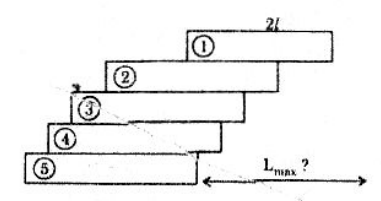
\includegraphics[scale=1.2]{../figs/VN10-2021-PH-TP023-1.png}
		\end{center}
	Mép bên phải của thanh thứ nhất và thanh thứ năm có thể cách xa nhất là bao nhiêu để thanh vẫn không bị đổ? Biết trọng tâm của mỗi thanh chính là tâm hình học của mỗi thanh.
	}
	
	\loigiai
	{		\begin{center}
			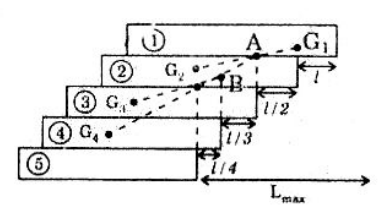
\includegraphics[scale=1.2]{../figs/VN10-2021-PH-TP023-2.png}
		\end{center}
	
		Ta xét lần lượt như sau:
		\begin{itemize}
			\item Thanh (1) không đổ khi trọng tâm $G_1$ nằm trên đường thẳng đi qua mép phải của thanh (2), khi đó mép phải của thanh (1) và mép phải của thanh (2) cách nhau $l$.
			\item Thanh (1) và (2) có trọng tâm chung là A, để hai thanh này không đổ thì A nằm trên đường thẳng đi qua mép phải của thanh (3), tức mép phải thanh (2) và mép phải thanh (3) cách nhau $l/2$.
			\item Thanh (1), (2), (3) có trọng tâm là B được xác định bởi $\dfrac{\text{BA}}{\text{BG}_3} = \dfrac{1}{2} \Rightarrow \text{BA} = \dfrac{1}{3} \text{AG}_3$. Vậy mép thanh (3) nhô ra $l/3$.
			\item Tương tự, tính được mép thanh (4) nhô ra $l/4$.
		\end{itemize}
	Vậy $L_\text{max} = l + l/2 + l/3 + l/4 = \dfrac{25}{12}l$.
	}
	\item \mkstar{4}
	
	\cauhoi
	{Một khối hộp có các cạnh $a=b=\SI{20}{cm}$, $c=\SI{30}{cm}$ đặt trên mặt phẳng nghiêng góc $\alpha$ so với mặt phẳng nằm ngang (hình vẽ).
		\begin{center}
			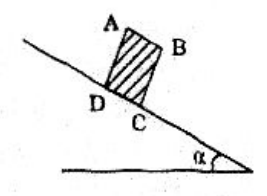
\includegraphics[scale=1]{../figs/VN10-2021-PH-TP023-3.png}
		\end{center}
	Hệ số ma sát trượt giữa khối hộp và mặt phẳng nghiêng là $\mu = \SI{0.7}{}$. Nghiêng dần mặt phẳng nghiêng để tăng góc $\alpha$. Hỏi khối hộp sẽ đổ trước hay trượt trước trong hai trường hợp sau?
	\begin{enumerate}
		\item Cạnh $a$ tiếp xúc với mặt phẳng nghiêng;
		\item Cạnh $c$ tiếp xúc với mặt phẳng nghiêng.
	\end{enumerate}
	}
	
	\loigiai
	{Trường hợp tổng quát:
		$$\vec P + \vec N + \vec F_\text{msn} = 0$$
		Suy ra:
		\begin{cases}
			P \sin $\alpha$ - F_\text{msn} =0 \\
			-P \cos $\alpha$ + N = 0
		\end{cases}
	Suy ra $F_\text{msn} = P \sin \alpha$, $N=P \cos \alpha$
	
	Với $F_\text{msn} \leq \mu N \Rightarrow \mu \geq \dfrac{F_\text{msn}}{\tan \alpha} \Rightarrow \mu \geq \tan \alpha$.
	
	Vậy vật bắt đầu trượt khi $\tan \alpha = \mu = \SI{0.7}{}$.
			\begin{enumerate}
			\item Cạnh $a$ tiếp xúc với mặt phẳng nghiêng;
			
	\begin{center}
		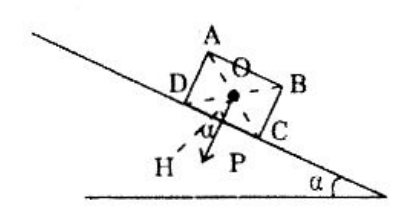
\includegraphics[scale=1]{../figs/VN10-2021-PH-TP023-4.png}
	\end{center}

	Ta biết vật sẽ đổ nếu giá của trọng lực $\vec P$ nằm ngoài mặt chân đế.
	
	Vật bắt đầu đổ khi $\tan \alpha' = \dfrac{\text{HC}}{\text{OC}} = \dfrac{a}{c} = \dfrac{2}{3} \Rightarrow \tan \alpha' < \tan \alpha$.
	
	Vậy vật sẽ đổ trước khi trượt.	
			\item Cạnh $c$ tiếp xúc với mặt phẳng nghiêng.
			
	Làm tương tự như trên, tính được $\tan \alpha'' = 1,5$. Suy ra $\tan \alpha'' > \tan \alpha$, vật sẽ trượt trước khi đổ.
		\end{enumerate}
	}
\end{enumerate}